\section{Systemtest}
\label{sec:systemtest}

In den Abschnitten \ref{subsec:tdd} und \ref{subsec:testframe} wurden Testgetriebene Entwicklung sowie die Testing Frameworks JSpec und Cucumber dargestellt. Im Folgenden wird die Umsetzung einer Testsuite mit diesen Technologien beschrieben.


\subsection{Unit Tests}
\label{subsec:unittests}

Das in Abschnitt \ref{subsec:jspec} vorgestellte Unit Test Framework JSpec wurde eingesetzt, um die Logik von Fachklassen und Helpern umfangreich zu testen. Die Tests sind je nach Modul und Funktionalität in mehrere Dateien aufgeteilt. In den Dateien sind Tests für folgende Funktionen enthalten: 

\begin{description}
  \item[note\_element\_spec:] Traversierung und automatische Speicherung der Zeilen
  \item[inserting\_note\_element\_spec:] Einfügen der Zeilen
  \item[indenting\_note\_element\_spec:] Einrücken der Zeilen
  \item[unindenting\_note\_element\_spec:] Ausrücken der Zeilen
  \item[focusing\_note\_element\_spec:] Setzen des Fokus beim Navigieren im Gliederungseditor
  \item[rendering\_note\_element\_spec:] Darstellung der Baumstruktur beim Öffnen eines Outlines
  \item[outline\_spec, outline\_helpers\_spec:] Sortierung und Darstellung der Outlines
  \item[note\_spec, note\_collection\_spec:] Auffinden bestimmter Zeilen beim Rendern eines Outlines
  \item[resources\_spec:] Abstraktion der Datenbankoperationen
  \item[lib\_spec:] Erweiterungen für die Datentypen String und Array
  \item[conflict\_spec:] Darstellung der Zeile beim Lösen eines Write-Konflikts
\end{description}
  

Die Testsuite wird ausgeführt, indem die Datei {\fontfamily{pcr}\selectfont /\_attachments/spec/index.html} im Browser geladen wird. Die Datei ist in Listing \ref{code:jspec-index} dokumentiert. In ihr werden zuerst die  JSpec-Bibliotheken geladen: das Testing Framework und der Programmcode, der getestet werden soll oder für die Ausführung des zu testenden Codes benötigt wird. Danach wird die Funktion {\fontfamily{pcr}\selectfont runSuites()} definiert. Darin wird auf dem {\fontfamily{pcr}\selectfont JSpec}-Objekt, das durch die Einbindung der JSpec-Bibliothek vorhanden ist, die Methode {\fontfamily{pcr}\selectfont exec} jeweils einmal mit jeder der oben genannten Dateien als Parameter aufgerufen. 

Zuletzt wird das Ausführen der Tests und die Ausgabe der Ergebnisse angestoßen. Dabei wird die Information über die Position der \textit{Fixtures} mit angegeben. Fixtures sind Dateien, die HTML-Blöcke enthalten. Da die JSpec-Tests nicht auf der Datenbank operieren, sondern nur die Javascript-Funktionen testen, wird auf diese Weise das DOM in einem bestimmten Zustand simuliert. Im Verzeichnnis {\fontfamily{pcr}\selectfont /\_attachments/spec/fixtures} liegen Fixtures, die Outlines in mehreren Zuständen sowie eine HTML-Repräsentierung der Startseite enthalten. Die Tests arbeiten mit diesen HTML-Seiten wie der Produktionscode mit dem generierten DOM. 

Die Ausgabe der Testergebnisse erfolgt im Browser. In der Ausgabe enthalten sind ggf. Informationen über fehlerhafte Tests, die Anzahl der Tests sowie die Laufzeit, die in Abbildung \ref{fig:jspec-good} etwas über drei Sekunden beträgt.

\medskip
\begin{figure}[ht] 
  \begin{center}
    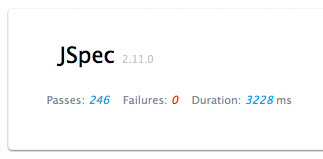
\includegraphics[width=0.5\textwidth]{grafik/jspec-example-good} 
  \end{center}
  \caption{JSpec: Erfolgreiche Ausführung aller Unit Tests}
  \label{fig:jspec-good} 
\end{figure}





\subsection{Integration Tests}
\label{subsec:integrationtests}

Das Framework Cucumber wurde bereits in Abschnitt \ref{subsec:cucumber} vorgestellt. Es wird üblicherweise mit der Bibliothek \textit{Webrat} \cite{webrat:website} verwendet. Webrat implementiert einen Browser-Simulator, der allerdings kein JavaScript beherrscht. Da die erstellte Anwendung komplett in JavaScript geschrieben ist, musste bei der Umsetzung der Integration Tests auf ein Setup aus \textit{HTMLUnit} \cite{htmlunit:website}, \textit{Culerity} \cite{celerity:website} und \textit{Celerity} \cite{culerity:website} zurückgegriffen werden. 

HTMLUnit ist eine Java-Bibliothek, die HTML parsen sowie JavaScript ausführen kann. HTMLUnit wird oft als ein \textit{headless browser (kopfloser Browser)} bezeichnet \cite{culerity:introduction}, da es über die Fähigkeiten eines Browsers verfügt, aber keine Benutzeroberfläche hat, in der die Seiten dargestellt werden. Die von HTMLUnit gelesenen bzw. ausgeführten Webseiten werden also nirgends angezeigt. Für die Ausführung der Testsuite ist HTML mindestens in Version 2.7 erforderlich. 

Celerity ist ein JRuby-Wrapper um HTMLUnit. Es bietet eine API für die am häufigsten verwendeten Browser-Funktionen, die dann auf HTMLUnit ausgeführt werden. Culerity ist ein Ruby-Gem, das Cucumber mit Celerity verbindet, auch wenn der Code nicht in einer JRuby-Umgebung ausgeführt wird. Bei der Verwendung mit Culerity erzeugt Celerity einen Java-Prozess, an den alle Celerity-Aufrufe weitergeleitet werden. Die Ergebnisse werden in der Ruby-Umgebung genau so ausgegeben, wie wenn sie von einem einzigen Ruby-Prozess erzeugt worden wären \cite{culerity:introduction}.

Culerity liefert eine Reihe häufig verwendeter Step-Definitionen mit. Diese liegen in der Datei {\fontfamily{pcr}\selectfont /features/step\_definitions/common\_culerity\_steps.rb}. Die weiteren Step-Definitionen sind im selben Verzeichnis zu finden. 

In Abschnitt \ref{subsec:cucumber} wurden bereits Beispiele für Features/Szenarios (s. Abschn. \ref{lst:cucumber-feature}) und Step-Definitionen (s. Abschn. \ref{lst:cucumber-steps}) angegeben. Diese sind der Testsuite für die Anwendung entnommen. Die weiteren Features sind im Ordner {\fontfamily{pcr}\selectfont /features} gespeichert. Der erfolgreiche Durchlauf aller Szenarios wird durch Abbildung \ref{fig:cucumber-good} veranschaulicht. Die Laufzeit beträgt etwa eineinhalb Minuten. Getestet werden die Funktionen: Outline anlegen und löschen; Titel eines Outlines ändern; zeitliche Sortierung der Outlines in der Übersicht; Zeile einfügen, bearbeiten, ein- und ausrücken. 


\medskip
\begin{figure}[ht] 
  \begin{center}
    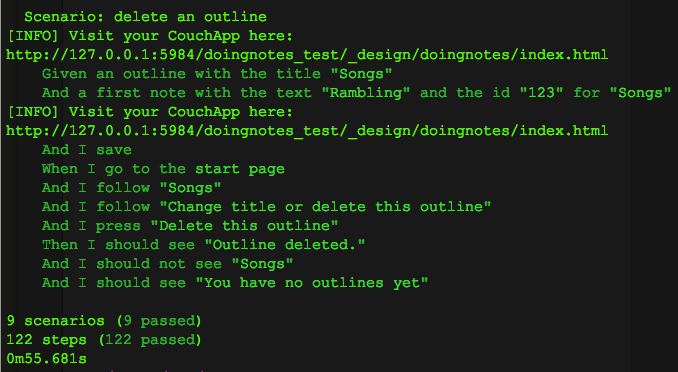
\includegraphics[width=\textwidth]{grafik/cucumber-example-good} 
  \end{center}
  \caption{Cucumber: Alle Tests laufen durch}
  \label{fig:cucumber-good} 
\end{figure}

Culerity betrachtet eine Änderung im Anker der URL nicht als Seitenwechsel. Damit dies richtig wahrgenommen wird und auch Sammy-Routen mit Cucumber getestet werden können, muss bei einer Änderung des Teils der URL nach dem Anker explizit die entsprechende Route aufgerufen werden. Da dieser Eingriff in die Funktionsweise von Sammy jedoch die Rückwärtsfunktion des Browsers deaktiviert, wird das Verhalten nur in der Testumgebung überschrieben. Deswegen wird im jeweils ersten Step eines Szenarios mit \lstinline!$browser.execute_script("setTestEnv();")! die in der Datei {\fontfamily{pcr}\selectfont test\_environment.js} enthaltene Funktion {\fontfamily{pcr}\selectfont setTestEnv()} aufgerufen, die die Testumgebung entsprechend setzt. Auf diese Weise können die Integration Tests ausgeführt werden, ohne dass das Verhalten der Anwendung beeinträchtigt wird. 






\subsection{Testsuite für die CouchDB HTTP-API}
\label{subsec:testsuite}

Die Anwendung wurde mithilfe der JavaScript-HTTP-API von CouchDB entwickelt. Diese API ist ein Wrapper um die grundlegenden Datenbankfunktionen, die den Entwicklern das Formulieren der Anfragen an die Datenbank erleichtert. Anfragen können als einfache JavaScript- bzw. jQuery-Methodenaufrufe erfolgen, ohne dass eigens ein XMLHttpRequest erzeugt werden muss. Da bislang keine Tests für die API vorlagen und Teile der API offensichtlich fehlerhaft waren, wurde eine Testsuite implementiert. Diese wird demnächst unter der Apache Lizenz veröffentlicht \cite{jira:testsuite}. Beispiele aus API und Testsuite finden sich in Abschnitt \ref{subsec:httpapi}. Des Weiteren wurden Verbesserungen an der API vorgenommen \cite{jira:bulkdelete, jira:bulksave}.

Die API-Tests werden, genau wie die Testsuite für die erstellte Anwendung, im Browser ausgeführt. Da sie im Gegensatz zu der oben beschriebenen Testsuite auf die Datenbank zugreifen, müssen sie von dieser ausgeliefert werden. Die Dateien können also nicht einfach im Browser geöffnet werden, sondern müssen in das Verzeichnis {\fontfamily{pcr}\selectfont /share/www} der CouchDB-Installation gelegt und mit dieser kompiliert werden. So sind die Tests, ähnlich wie Futon, unter der URL \url{http://localhost:5984/\_utils/spec/run.html} erreichbar.























\section{Deployment mit Amazon Web Services}

Die Anwendung soll nicht nur, wie in der Einleitung (Abschnitt \ref{sec:motivation}) ausgeführt, \enquote{nach unten skalieren}, sondern ebenfalls eine hohe Performance bieten: Auch wenn eine große Anzahl von Benutzern ihre Outlines zum selben Zeitpunkt über einen Server sychronisieren möchten, soll dies ohne Latenzerhöhung stets möglich sein. Wenn die CouchDB-Instanz auf dem Server einmal zeitweise nicht verfügbar ist, soll die Verfügbarkeit trotzdem gegeben sein. Mit Amazon Web Services lässt sich dies problemlos umsetzen.

Im Rahmen der Entwicklung des Prototypen wurde deshalb evaluiert, wie ein Deployment mit der \textit{Amazon Elastic Compute Cloud (EC2)} umgesetzt werden kann. Die technischen Hintergründe von Cloud Computing wurden bereits in Abschnitt \ref{sec:cloud} dargestellt. Im Folgenden soll ein Überblick über die Konfiguration einer über EC2 deployten Anwendung gegeben werden. Die Darstellung stützt sich auf eigene Recherchen sowie auf \citelit[Kap. 4.1]{cloud:cloudcomputing}.

AWS ist der Sammelbegriff für alle Cloud-Computing-Angebote der Firma Amazon. Amazon hat starke saisonale Schwankungen in der Nachfrage nach seinen Angeboten. Deswegen wird der Großteil der erheblichen IT-Ressourcen die meiste Zeit über nicht genutzt. Das AWS-Angebot resultiert aus der Geschäftsidee, die freien Ressourcen gegen Entgelt zur Verfügung zu stellen, wenn sie temporär nicht für eigene Produkte benötigt werden.

Mit EC2 kann der Benutzer über Web Services virtuelle Server verwalten. Um einen solchen Server einzurichten, müssen eine Reihe von Schritten ausgeführt werden. Diese Schritte sind im Anhang (Abschnitt \ref{subsec:aws}) mithilfe von Screenshots genauer dokumentiert.

Nach dem Erstellen des Amazon-Accounts wird zunächst ein \textit{Schlüsselpaar} generiert, mit dem eine Identifizierung gegenüber der EC2-Instanz möglich ist (s. Abb. \ref{fig:aws-key}). Der öffentliche Schlüssel wird mit dem Amazon-Account assoziiert, der private verbleibt auf dem Rechner des Benutzers.

Auch muss eine \textit{Security Group} definiert und konfiguriert werden (s. Abb. \ref{fig:aws-group}). Jede EC2-Instanz gehört einer solchen Security Group an. Über diese werden die Sicherheitseinstellungen definiert. Mit dem Public Key aus dem vorherigen Schritt können einzelne Ports freigeschaltet werden, über die auf den Server zugegriffen werden kann. 

Des Weiteren muss die \textit{Availability Zone} ausgewählt werden, also die geographische Region, auf der der Server laufen soll. Bei großen Installationen ist eine Verteilung auf unterschiedliche Zonen vorteilhaft, um gegen den Ausfall einer Region abgesichert zu sein. Mit einer optimalen Availability Zone kann außerdem die Latenz gering gehalten werden.

Nun wird die \textit{Größe der Ressourcen} des Servers festgelegt (s. Abb. \ref{fig:aws-size}). Es stehen verschiedene Pakete zur Verfügung, die sich in der Leistungsfähigkeit des Prozessors und in der Größe des Arbeitsspeichers sowie der Festplatte unterscheiden. Das Spektrum des Angebots erstreckt sich von 1,7 GB RAM / 160 GB Festplattenspeicher bis hin zu 68,4 GB RAM / 1690 GB Festplattenspeicher \cite{aws:instances}.

Zuletzt muss ein \textit{Amazon Machine Image (AMI)} ausgewählt werden (s. Abb. \ref{fig:aws-ami}). Ein AMI ist virtuelles Image, also eine Art Blaupause eines virtuellen Servers. Die AMIs unterscheiden sich bezüglich des Betriebssystems und der auf ihnen installierten Software-Pakete. Eigene Images können zur späteren Wiederverwendung angefertigt und auch gegen oder ohne Entgelt veröffentlicht werden. Für Testzwecke genügt es, den virtuellen Server aus einem vorgefertigten AMI zu erstellen. Gewählt wird eine aktuelle Ubuntu-Distribution, \enquote{alestic's 64bit server Ubuntu 9.04 AMI} mit der ID \enquote{ami-ccf615a5}.

Die EC2-Instanz wird mit den oben festgelegten Parametern gestartet. Der neu entstandene virtuelle Server erhält automatisch eine öffentliche IP, unter der er im Internet erreichbar ist, und eine private, über die er mit anderen Instanzen kommunizieren kann. Diese IPs werden bei jedem Start neu vergeben. Deswegen ist zu empfehlen, eine \textit{Elastic IP} einzurichten (s. Abb. \ref{fig:aws-ip}). Wird diese statische IP mit dem Server verknüpft, hat er nach jedem Neustart immer wieder dieselbe IP.

Die Verwaltung der Instanz erfolgt im Allgemeinen über die \textit{AWS Management Console} (s. Abb. \ref{fig:aws-console}). Diese ist unter der Adresse \url{https://console.aws.amazon.com/ec2/home} erreichbar. Die Verwaltung kann auch über Kommandozeilenbefehle erfolgen. Ist die Instanz bspw. unter der IP {\fontfamily{pcr}\selectfont 184.73.233.128} erreichbar, und ist der Public Key in der Datei {\fontfamily{pcr}\selectfont .ssh/doingnotes.pem} abgelegt, ist ein Login in die Instanz mit dem Befehl \lstinline!ssh -i .ssh/doingnotes.pem root@ec2-184-73-233-128.compute-1.amazonaws.com! möglich. Ist der Server eingerichtet, wird CouchDB wie auf einem normalen Ubuntu-Rechner installiert (siehe Anleitung in Abschnitt \ref{sec:installation}).

Wird die Instanz einmal beendet, werden alle Einstellungen und Installationen, die darauf vorgenommen wurden, gelöscht. Um Änderungen auch über die Laufzeit eines virtuellen Servers hinweg zu persistieren, muss der Zustand der Instanz extern gespeichert werden. Dafür kann \textit{Amazon Elastic Block Store (EBS)} verwendet werden (s. Abb. \ref{fig:aws-ebs}). Ein EBS wird nach dem Erstellen wie eine externe Festplatte als Laufwerk mit der EC2-Instanz verknüpft. Darauf können Momentaufnahmen des EC2-Servers gespeichert werden.

Die Kosten für eine EC2-Instanz richten sich nach der Leistungsfähigkeit des Servers und werden stundenweise abgerechnet. Der Preis setzt sich aus der Größe der Ressourcen, dem Volumen der Datentransfers und der Zeit der Verwendung von Elastic IPs und EBS zusammen. Unter \cite{aws:preistabelle} lassen sich die Kosten für das gewünschte Paket im Voraus berechnen.



\section{Clustering mit Couchdb-Lounge}
\label{subsec:lounge}


Im folgenden Abschnitt wird beschrieben, wie die Verteilung eines Systems auf mehrere CouchDB-Instanzen möglich ist, ohne dass sich für Benutzer des Systems etwas ändert. Für diesen Zweck kommt CouchDB-Lounge \cite{lounge:website} zum Einsatz. CouchDB-Lounge ist eine Proxy-basierte Anwendung für \textit{Clustering} und \textit{Partitionierung} \cite{lounge:SOC}. Diese beiden Konzepte können helfen, die Verfügbarkeit bzw. die Leistung eines
Systems zu erhöhen.

Clustering wurde bereits im Jahr 1997 als Lösungsansatz empfohlen, den steigenden Anforderungen von modernen Datenbankanwendungen nachzukommen \citelit{dataplacement}. Ein Computer-Cluster bezeichnet allgemein eine Anzahl ...

\begin{quote}
... ähnlicher Arbeitsstationen oder PCs, die mithilfe eines lokalen Hochgeschwindigkeitsnetzwerkes miteinander verbunden sind. \citelit[S. 34]{tanenbaum:vs}
\end{quote}

Im konkreten Fall beschreibt Clustering den redundanten Einsatz mehrerer CouchDB-Server, um \textit{Lastverteilung (Load-Balancing)} und erhöhte Verfügbarkeit zu ermöglichen. Mehrere CouchDB-Instanzen laufen parallel; Anfragen werden gleichmäßig auf die Instanzen verteilt. Daten redundant zu speichern, damit im Fall eines Hardware-Ausfalls immer mehrere Kopien der Daten bereitstehen, kann ebenfalls mit CouchDB-Lounge umgesetzt werden. Dies wird im Rahmen dieser Arbeit jedoch nicht detaillierter ausgeführt.

Horizontale Partitionierung ist die Praxis, den Speicherplatz auf Partitionen aufzuteilen. Diese werden als \textit{Shards} bezeichnet. Die Shards werden auf Server verteilt, um den Durchsatz zu erhöhen. Dadurch wird verhindert, dass die Performance der Festplatten zum Bottleneck wird. Im nächsten Abschnitt wird dies näher beschrieben.

\subsection{Funktionsweise}

CouchDB-Lounge ist eine neue Technologie, weder ihre Funktionsweise noch ihr Einsatz sind bisher gut dokumentiert. Die folgende Darstellung bezieht sich daher im Wesentlichen auf \citelit[Kap. 19]{couchdb}, und \cite{lounge:wiki}.

Lounge besteht aus zwei Hauptkomponenten. Ein \textit{Smartproxy} behandelt CouchDB-Views und verteilt sie auf die anderen Knoten im Lounge-Cluster. Die Performance der Views kann demnach durch eine Erhöhung der Anzahl der Knoten im Cluster gesteigert werden. Der Smartproxy ist als Daemon für \textit{Twisted} implementiert, ein \enquote{framework for writing asynchronous, event-driven networked programs in Python} \cite{twisted}. Ein \textit{Dumbproxy} ist ein Modul für \textit{nginx}, ein Webserver und Reverse Proxy Server. Der Dumbproxy wird eingesetzt, um GET- und PUT-Requests entgegenzunehmen, die nicht an CouchDB-Views gerichtet sind. Auch diese Requests werden auf die einzelnen Knoten verteilt. Dabei wird den Clients der Eindruck vermittelt, es handle sich um eine einzige CouchDB-Installation. Beide Module arbeiten mit eindeutigen Hashes, die CouchDB-Lounge aus den IDs der CouchDB-Dokumente bildet. Anhand der ersten Zeichen des hexadezimal dargestellten Hashes wird der Shard ausgewählt, dem dieses Dokument zugewiesen wird. Die genaue Zuteilung wird in einer \textit{Shard-Map} konfiguriert.

Mit CouchDB-Lounge kann also ein Cluster erstellt werden, das nach außen unter einer Adresse erreichbar ist. Der Cluster wird in Abbildung \ref{fig:lounge-scaling1} als Ring dargestellt. Den einzelnen der acht Knoten sind jeweils zwei Shards zugeteilt, denen wiederum jeweils eine Ziffer aus dem Hexadezimalsystem zugewiesen ist. Beginnt der Hash einer ID eines CouchDB-Dokuments mit dieser Ziffer, speichert Lounge dieses Dokument in den entsprechenden Shard. Durch das Verfahren werden HTTP-Requests zu dem tatsächlichen Speicherort des Dokuments weitergeleitet. So kann eine Partitionierung umgesetzt werden.
 
\medskip
\begin{figure}[H] 
  \begin{center}
    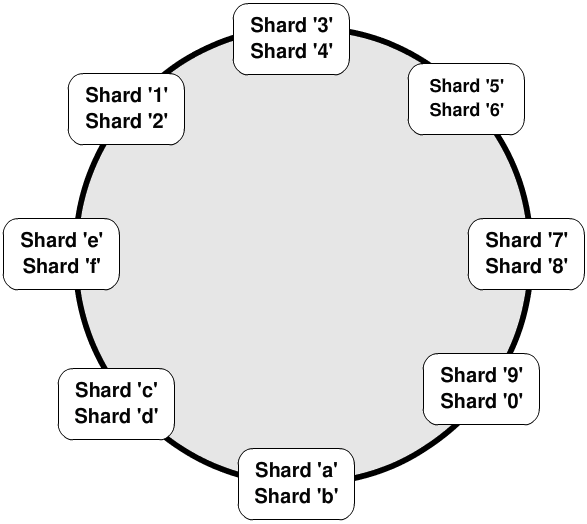
\includegraphics[width=0.6\textwidth]{grafik/shards1} 
  \end{center}
  \caption[16 Shards, 8 Knoten]{16 Shards, 8 Knoten. Nach \citelit{nosql:jan}}
  \label{fig:lounge-scaling1} 
\end{figure}

\begin{quote}
From the outside world, a couchdb lounge cluster looks just like any other couchdb node. [...] There's no difference from a functional perspective. [...] Its sharded nature is completely transparent. \cite{lounge:blogpost}
\end{quote}

Ist zu erwarten, dass die Anforderungen an die Kapazität des Systems während seiner Lebensdauer steigen, wird in \citelit{couchdb} und \cite{lounge:till} empfohlen, die Anzahl der Shards zu Beginn möglichst hoch zu wählen. Die Daten auf mehr Shards zu verteilen, als Knoten verfügbar sind, wird \enquote{Oversharding} genannt. Auch wenn eine geringe Anzahl Knoten zu Beginn ausreicht, kann diese später beliebig erhöht werden, indem weitere Knoten hinzugefügt werden. Die Shards werden dann auf diese verteilt. Dies wird in Abbildung \ref{fig:lounge-scaling1} skizziert. Das System in Abbildung \ref{fig:lounge-scaling1} hat seine Schnittstelle behalten, die CouchDB-Installationen auf den Knoten wurden allerdings jeweils durch Lounge-Konfigurationen ersetzt. Sollen weitere Shards nachträglich hinzugefügt werden, muss der gesamte Cluster neu aufgebaut werden.

\medskip
\begin{figure}[H] 
  \begin{center}
    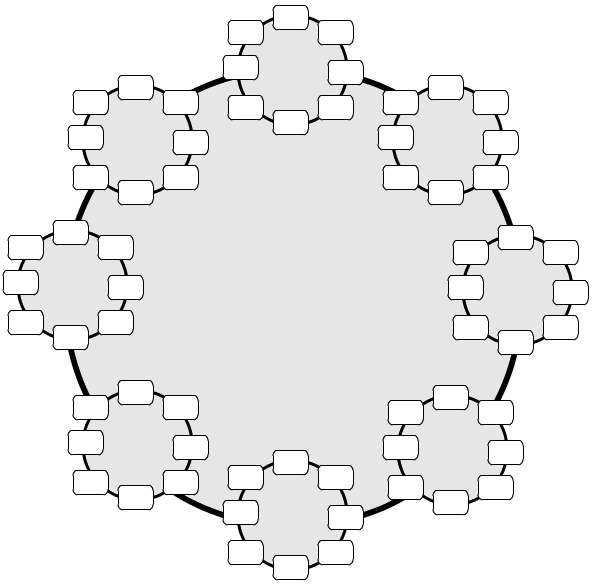
\includegraphics[width=0.6\textwidth]{grafik/shards2} 
  \end{center}
  \caption[16 Shards, 8 Knoten mit je 16 Sub-Shards, 8 Subknoten]{16 Shards, 8 Knoten mit je 16 Sub-Shards, 8 Subknoten. Nach \citelit{nosql:jan}}
  \label{fig:lounge-scaling2} 
\end{figure}

Auch für kleinere Projekte besteht bei Oversharding der Vorteil, dass aufgrund der geringeren Anzahl der Dokumente die Größe des Index klein bleibt, und alle Operationen dadurch schneller ausgeführt werden können. 


\subsection{Konfiguration}
\label{subsec:lounge-install}

In \cite{lounge:website} findet sich der Quelltext von CouchDB-Lounge. Er enthält Anweisungen, wie Dumbproxy, Smartproxy und \textit{Python-Lounge}, eine Sammlung von benötigten Modulen, installiert werden müssen. In der aktuellen Version von CouchDB-Lounge besteht eine Abhängigkeit zu CouchDB in der Version 0.10.0. Nur für diese Version liegt ein Patch vor, der die benötigte \enquote{design-only replication} aktiviert \cite{lounge:wiki}. In späteren Versionen von CouchDB wird dieses Feature aber bereits vorinstalliert sein. 

In \cite{lounge:twoinstances} ist beschrieben, wie auf einem Rechner mehrere CouchDB-Instanzen installiert werden können. Die zentrale CouchDB-Konfigurationsdatei in {\fontfamily{pcr}\selectfont /etc/couchdb/local.ini} muss so oft kopiert werden, wie Instanzen laufen sollen. Listing \ref{lst:local.ini} beinhaltet die wichtigen Teile aus der Kopie in {\fontfamily{pcr}\selectfont local-1.ini}. In den Kopien in {\fontfamily{pcr}\selectfont local-2.ini} etc. müssen die Angaben zu Port und Logfile entsprechend angepasst werden.
 
\medskip
\begin{lstlisting}[caption=Auszug aus der CouchDB Konfigurationsdatei, label=lst:local.ini]
[httpd] 
port = 5984
bind_address = 127.0.0.1

[log]
file = /var/log/couchdb/couch-1.log
\end{lstlisting}


Listing \ref{lst:startcouch} zeigt, wie die erste CouchDB-Instanz auf einem Unix-System (Mac OS X 10.6) gestartet werden kann:

\medskip
\begin{lstlisting}[caption=Starten einer CouchDB-Instanz, label=lst:startcouch]
sudo -i -u couchdb '/usr/local/bin/couchdb -a etc/couchdb/local-1.ini -p /usr/local/var/run/couchdb/couchdb-1.pid -o /usr/local/var/log/couchdb/error-1.log -e /usr/local/var/log/couchdb/error-1.log -b'
\end{lstlisting}

Ist die gewünschte Anzahl an CouchDB-Knoten eingerichtet und gestartet, wird die Funktionsfähigkeit des Setups überprüft, indem die CouchDB-Testsuite wie in der Installationsanleitung angegeben ausgeführt wird. Läuft die Testsuite fehlerfrei durch, muss CouchDB-Lounge vor der Benutzung konfiguriert werden. Dies geschieht durch Anpassung der Datei \url{/var/lounge/etc/shards.conf}. Darin wird die Anzahl der Shards und der Grad der Redundanz definiert. Die Datei enthält das JSON-Objekt {\fontfamily{pcr}\selectfont nodes}, in dem Informationen über die Anzahl der CouchDB-Knoten gespeichert sind. Jeder Eintrag in dem Array enthält den Hostnamen und den Port eines Knoten. Die {\fontfamily{pcr}\selectfont shard\_map} ist ein Array aus Arrays, in dem bestimmt wird wo sich ein Shard befindet und wohin es repliziert werden soll. Die Anzahl der Shards und Knoten kann beliebig hoch gesetzt und beliebig redundant ausgelegt werden. 

Listing \ref{lst:shardsconf} beschreibt zwei Shards auf zwei Knoten, von denen das erste Shard (mit der Nummer 0) sich auf Knoten 0 befindet, das zweite (mit der Nummer 1) sich auf Knoten 1. Das erste wird zu Knoten 1 repliziert, wenn Knoten 0 ausfallen sollte, und umgekehrt.

\lstset{language=bash}
\medskip
\begin{lstlisting}[caption=shards.conf mit zwei Knoten und einfacher Redundanz, label=lst:shardsconf]
{
  "shard_map": [[0,1], [1,0]],
  "nodes": [ ["localhost", 5984], ["localhost", 5985] ]
}
\end{lstlisting}

Listing \ref{lst:shardsconf-long} definiert einen Cluster mit acht Shards auf vier Knoten ohne Redundanz. Die Knoten auf beiden Beispielen liegen auf demselben Rechner, sie könnten aber auch durch Angabe eines anderen Hostnamen auf mehrere Maschinen verteilt werden.

\medskip
\begin{lstlisting}[caption=shards.conf mit vier Knoten ohne Redundanz mit einfachem Oversharding, label=lst:shardsconf-long]
{
  "shard_map": [[0], [1], [2], [3], [0], [1], [2], [3]],
  "nodes": [ ["localhost", 5984], ["localhost", 5985], ["localhost", 5986], ["localhost", 5987]] ]
}
\end{lstlisting}

CouchDB-Lounge ist erfolgreich installiert und konfiguriert, wenn ein auf einem Knoten erstelltes Dokument automatisch auf all die Knoten kopiert wird, für die in {\fontfamily{pcr}\selectfont shard\_map} Redundanz definiert ist. 

